\documentclass[a4paper]{article}
\usepackage{xeCJK}
\usepackage{geometry}
\geometry{left=2.5cm,right=2.5cm,top=3cm,bottom=3cm}
\title{Algorithm Homework 4}
\author{龙肖灵 \\Xiaoling Long\\Student ID.:81943968\\email:longxl@shanghaitech.edu.cn}
\usepackage{graphicx}
\usepackage[colorlinks,linkcolor=red]{hyperref}
\usepackage{amsmath, amsthm, amssymb}
%\usepackage{subfloat}
\usepackage{float}
\usepackage{setspace}
\usepackage{enumerate}
\usepackage{colortbl}
\usepackage{multirow}
\usepackage{tikz}
\usetikzlibrary{graphs}
\usetikzlibrary{quotes}
\usepackage{pgf}
\usepackage{listings}
\usepackage{subfigure}
%\usepackage[usenames,dvipsnames,svgnames,table]{xcolor}
\newtheorem{prop}{Proposition}
\usepackage{ulem}

\newenvironment{solution}
  {\renewcommand\qedsymbol{$\blacksquare$}\begin{proof}[Solution]}
  {\end{proof}}

\renewcommand{\baselinestretch}{1.2}

\definecolor{light-gray}{gray}{0.7}
\usepackage{indentfirst}
\lstset{% general command to set parameter(s)
basicstyle=\ttfamily,frame=tlb,backgroundcolor=\color{light-gray},breaklines}

\begin{document}
\maketitle

\paragraph{Note:}When proving problem $A$ is NP-complete, please clearly divide your answer into three steps:
\begin{enumerate}[(1)]
  \item Prove that problem $A$ is in $NP$.
  \item Choose an NP-complete problem $B$ and for any $B$ instance, construct an instance of problem $A$.
  \item Prove that the yes/no answers to the two instances are the same.
\end{enumerate}


\section*{Problem 1}
\paragraph{}
Given a conjunctive normal form formula and an integer $k$, can this formula be satisfied by an assignment
in which at most $k$ variables are true? Prove this problem is NP-complete.

\begin{solution}\
  \begin{enumerate}[(1)]
    \item Certification: Give an assignment in which less than or equal $k$ variable are true. We can certify this problem whether this formula is satisfied. So, this problem is NP.
    \item Reduction $1$: First of all, $3-SAT$ is a special case of this problem when $k=n$. If we can solve this problem. We can solve all $3-SAT$ problem. So $3$-SAT $\le_{p} CNF_{k}$
    \item Reduction $2$: And Similarly, we can construct an instance of $CNF_{k}$ from any circuit instance.
    \begin{enumerate}[Step 1:]
      \item Create a $CNF_{k}$ variable $x_{i}$ fpr each circuit element $i$.
      \item Convert all logical predicates into $\lor$:
      \begin{itemize}
        \item $x=\neg y$\quad $\Rightarrow$\quad $x\lor y,\  \bar{x}\lor \bar {y}$
        \item $x=y\lor z$ \quad $\Rightarrow$\quad  $x\lor \bar{y}$,\ $x\lor\bar{z}$,\ $\bar{x}\lor y \lor z$
        \item $x=y\land z$ \quad $\Rightarrow$\quad $\bar{x}\lor y$,\ $\bar{x}\lor z$,\ $x\lor \bar{y}\lor \bar{z}$
      \end{itemize}
      \item Set output value and input value. If it is $1$, then $x$, or not $\neg x$
      \item Then $CNF_{k}$ consist of all of clauses.
    \end{enumerate}
    \item Proof(2): So if  this formula can be satisfied by an assignment when $k=n$, the CIRCUIT-SAT can be satisfied, since output value equals to $1$. Or not, the CIRCUIT-SAT cnnot be satisfied. And if CIRCUIT-SAT can be satisfied, our construction ensures that all the nodes in CIRTUIT-SAT are correctly coputed an the output is $1$, the $CNF_{k}$ can be satisfied as well.
    \item Conclusion: CIRCUIT-SAT$\le_{p}CNF_{k}$. This problem $CNF_{k}$ is NP-complete.
  \end{enumerate}
  Done.
\end{solution}

\section*{Problem 2}
\paragraph{}
Textbook Chapter 8 Exercises 17 (Note: You must use the Directed-Hamiltonian-Cycle problem in your
reduction.)
You are given a directed graph $G = (V, E)$ with weights we on its edges $e \in E$. The weights can be
negative or positive. The Zero-Weight-Cycle Problem is to decide if there is a simple cycle in $G$ so that the
sum of the edge weights on this cycle is exactly $0$. Prove that this problem is NP-complete.

\begin{solution}\
  \begin{enumerate}[(1)]
    \item Certification: Given a cycle, we can add all weights to check whether this circle is a ZERO-Weight-Cycle or not. So Zero-weight-Cycle problem is NP.
    \item Construction: Split each directed edge into $2$ edges from any Directed-Hamiltonian-Cycle instance $G$ and the weights of the edges are $1$ and $-1$ respectively. Such as there exists an edge $(u,v)\in E$.
    \begin{center}
      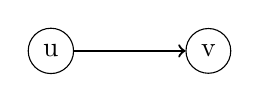
\begin{tikzpicture}[every edge quotes/.style={fill=white,font=\footnotesize}]


        \node[circle,draw]         (u) at (-1, 0)              {u};
        \node[circle,draw]         (v) at (1, 0)           {v};

        \draw (u) edge[ ->,thick]  (v);
      \end{tikzpicture}
    \end{center}
    After splitting, we have sub-graph in $G^{\prime}$ as following,
    \begin{center}
      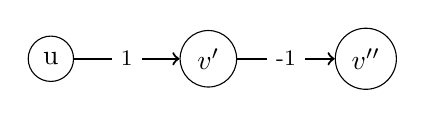
\begin{tikzpicture}[every edge quotes/.style={fill=white,font=\footnotesize}]


        \node[circle,draw]         (u) at (-2, 0)              {u};
        \node[circle,draw]         (v1) at (0, 0)           {$v^{\prime}$};
        \node[circle,draw]         (v2) at (2, 0)           {$v^{\prime\prime}$};

        \draw (u) edge["1", ->,thick]  (v1);
        \draw (v1) edge["-1", ->,thick]  (v2);
      \end{tikzpicture}
    \end{center}
    And all edges come into $v$ come into $v^{\prime}$  now, and all edges leave out leave from $v^{\prime\prime}$ now.
    \item Proof: If there is a cycle in $G$, then there must exist a cycle along with all node $v_{i}^{\prime}$ and $v_{i}^{\prime \prime}$, where $v_{i}$ are the nodes in the cycle in graph $G$.\\
    If there exists a Zero-Weight-Cycle in $G^{\prime}$, then we can also find a cycle in $G$ in same order.
    \item Conclusion: Directed-Hamiltonian-Cycle$\le_{p}$ Zero-Weight-Cycle. So Zero-Weight-Cycle problem is NP-complete.
  \end{enumerate}
  Done.
\end{solution}

\section*{Problem 3 }
\paragraph{}
Given a graph $G = (V, E)$, select a subset of the nodes such that for every node $v \in V$ , $v$ is selected or
at least one of its neighbors is selected. We would like to know if we can find such a subset of at most $K$
nodes. Show that this problem is NP-complete.


\begin{solution}\
  \begin{enumerate}[(1)]
    \item Certification: Given a subset, we can check whether all nodes can be satisfied. So this problme is NP.
    \item We can reduction from \bfseries Vertex Cover \mdseries .
    \item Construction: Construct a triangle based on each edge from \bfseries Vertex Cover ($G$)\mdseries. If there is an edge in $G$
    \begin{center}
      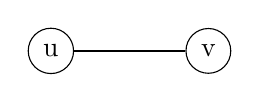
\begin{tikzpicture}[every edge quotes/.style={fill=white,font=\footnotesize}]


        \node[circle,draw]         (u) at (-1, 0)              {u};
        \node[circle,draw]         (v) at (1, 0)           {v};

        \draw (u) edge[ -,thick]  (v);
      \end{tikzpicture}
    \end{center}
    Then we add a nodes and two edges into $G^{\prime}$ as following,
    \begin{center}
      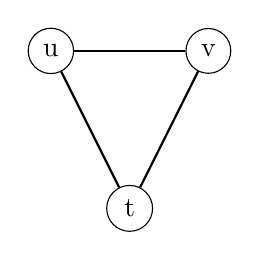
\begin{tikzpicture}[every edge quotes/.style={fill=white,font=\footnotesize}]


        \node[circle,draw]         (u) at (-1, 0)              {u};
        \node[circle,draw]         (v) at (1, 0)           {v};
        \node[circle,draw]         (t) at (0, -2)           {t};

        \draw (u) edge[ -,thick]  (v);
        \draw (v) edge[ -,thick]  (t);
        \draw (u) edge[ -,thick]  (t);
      \end{tikzpicture}
    \end{center}
    Then we can get the new graph $G^{\prime}$.
    \item Proof: If \bfseries Vertex Cover \mdseries can be satisfiede, then we can choose the same nodes in subset to satisfy the problem.\\
    If The graph $G^{\prime}$ can be satisfied, then in one trangle we at least selected a node, if we selected node $t$, we can selected any one of $u$ and $V$ in the problem \bfseries Vertex Cover ($G$) \mdseries. The \bfseries Vertex Cover \mdseries can be satisfied .
    \item Conclusion: Vertex Cover $\le_{p}$ Subset selection. This problem is NP-complete.
  \end{enumerate}
  Done.
\end{solution}

\section*{Problem 4}
\paragraph{}
Suppose you are going to schedule courses for the SIST and try to make the number of conflicts no
more than $K$. You are given $3$ sets of inputs: $C = \{\cdots\}, S = \{\cdots\}, R = \{\{\cdots\}, \{\cdots\}, \cdots\}$. $C$ is the set of
distinct courses. $S$ is the set of available time slots for all the courses. $R$ is the set of requests from students,
consisting of a number of subsets, each of which specifies the courses a student wants to take. A conflict
occurs when two courses are scheduled at the same slot even though a student requests both of them. Prove
this schedule problem is NP-complete.
Example:
$$K = 1; C = \{a, b, c, d\}, S = \{1, 2, 3\}, R = \{\{a, b, c\}, \{a, c\}, \{b, c, d\}\}$$
An acceptable schedule is:
$$a \to 1; b \to 2; c, d \to 3;$$
Here only one confilct occurs. An unacceptalbe schedule is:
$$a \to 1; b, c \to 2; d \to 3;$$
Here two ($> K$) conflicts occur.


\begin{solution}\
  \begin{enumerate}[(1)]
    \item Certification: Given a schedule, we can count the number of the confilct. So , this schedule problem is NP.
    \item We can reduction from $3$-Colorability problem.
    \item Construction: $C$ is the set of all nodes. $S$ is the set of 3 colors. If there exists an edge $(u,v)\in E$, it means that there is a student wants to take these two courses $u$ and $v$. And $K=0$.
    \item Proof: If the schedule problem can be satisfied, then there is no course a student wants to take in same slot. This ensure no adjacent nodes have the same color.\\
    If the $3$-Colorability can be satified, then all red nodes can be scheduled into slot $1$, blue into slot $2$, and green into slot $3$. And all students' courses at the different slots. The schedule problem can be satified as well.
    \item Conclusion: $3$-Colorability $\le_{p}$ Schedule Problem. So this schedule problme is NP-complete.
  \end{enumerate}
  Done.
\end{solution}

\section*{Problem 5}
\paragraph{}
A company has two trucks and must deliver a number of parcels to a number of addresses. They want
both drivers to be home at the end of the day. This gives the following decision problem:\\
  \bfseries Instance:\ \mdseries Set $V$ of locations; for each pair of locations $v, w \in V$ , an integer distance $d(v, w)$; a starting
  location $s \in V$ ; and an integer $K$.\\
  \bfseries Question:\ \mdseries Are there two cycles that both start at $s$, such that every location in $V$ is on at least one of the
  two cycles, and both cycles have length at most $K$?\\
  Show that this problem is NP-complete.\\
  \bfseries Note:\ \mdseries A cycle is a path $v_{1} , v_{2} , \cdots, v_{k-1}, v_{k}$ in which $v_{1} = v_{k}$ , $k > 2$, and the first $k − 1 $nodes are all distinct.


\begin{solution}\
  \begin{enumerate}[(1)]
    \item Certification: Given to cycles, we can chech whether this planning problem can be satisfied. So this planning problem is NP.
    \item We can reduction from HAMILTONIAN-CYCLE Problem. A Hamiltonian cycle can be splitted into $2$ isometric cycle after adding $2$ edges.
    \item Construction: Select any node in the $V$ as start node. Then add some edges which nodes isn't adjacent to $s$ and the weight is $2$.
    And the weight of all $(u,v)\in E$ is $1$. And $K=\lceil \frac{n}{2}\rceil+2$
    \item Proof: If HAMILTONIAN-CYCLE Problem can be satisfied, then we can start at $s$ and go throught same length or one is greater $1$ than another, then come back to $s$.\\
    If the planning problem can be satisfied, then delete the additional edges, connect the last nodes of two cycle. We can get the Hamiltonian cycle.
    \item Conclusion: HAMILTONIAN-CYCLE $\le_{p}$ Planning Problem. So this problem is NP-complete.
  \end{enumerate}
  Done.
\end{solution}

\section*{Problem 6}
\paragraph{}
Consider the Knapsack problem. We have $n$ items, each with weight $a_{j}$ and value $c_{j}\ (j = 1, \cdots, n)$. All
$a_{j}$ and $c_{j}$ are positive integers. The question is to find a subset of the items with total weight at most $b$ such
that the corresponding profit is at least $k$ ($b$ and $k$ are also integers). Show that Knapsack is NP-complete
by a reduction from \bfseries Subset Sum \mdseries .

\begin{solution}\
  \begin{enumerate}[(1)]
    \item Certification: Given a subset, we can certify whether this problem can be satisfied. So this knapsack is NP.
    \item Construcation: We can do some assignment as following $$c_{i}=1, a_{i}=w_{i}, i=1,\cdots,n\quad c_{n+1}=n, a_{n+1}=\sum_{i} w_{i}-W$$
    We also have $b=\sum_{i}w_{i}$  and $k=n+1$. If we can find a subset with total weight $b$ and the correspoding profit is at least $n+1$, then we can solve this \bfseries Subset Sum \mdseries.
    \item Proof: If This \bfseries Knapsack Problem \mdseries can be satisfied, then the subset of Knapsack without $a_{n+1}$ will be the solusiton of \bfseries Subse Sum \mdseries.\\
    If \bfseries subsection Sum \mdseries can be satisfied, then the construction ensure the knapsack can be satisfied.
    \item Conclusion: Subset Sum $\le_{p}$ Knapsack Problem. So this Knapsack Problem is NP-complete.
  \end{enumerate}
  Done.
\end{solution}

\end{document}
